成绩:平时(作业+考勤)+期中论文+期末

\section*{概率论准备知识}

概率论中,随机变量的本质是可测函数。

\[
X:\Omega\rightarrow S
\]

$S$ 的 $\sigma$-代数记为 $\mathcal{S}$,是个 Borel $\sigma$-代数(由开集/闭集生成)

Q: 为什么要给 $\Omega$ 一个$\sigma$-代数?

A: 样本空间是抽象的,给它$\sigma$-代数赋予它结构,相当于对信息进行重整/提取

概率测度的本质是集函数,

\[
\text{集合}\rightarrow \text{函数}
\]

将信息具象化,

\[
\begin{aligned}
    \PP: &\mathcal{F}\rightarrow [0,1]\\
    &A\rightarrow \PP(A)
\end{aligned}
\]

随机过程:一族随机变量 $\{X_t\}_{t\in \mathbb{T}}$

其中 $\mathbb{T}$ 为指标集,$X_t:\Omega\rightarrow S$

\begin{example}
$\mathbb{T}=\mathbb{N}_0$: 时间离散;$\mathbb{T}=[0,T]$: 时间连续 
\end{example}

\[
X:(\Omega, \mathcal{F}, \PP)\rightarrow (S,\mathcal{S}, \mu_X)
\]

思考:什么是随机过程的分布$\{\mu_t\}_{t\in \mathbb{T}}$?

\newpage

\subsection{事件概率}

\subsubsection{事件域}

\begin{definition}[样本空间、事件]
    样本点、样本空间、事件和事件的运算:
    \begin{itemize}
        \item 样本点 $\omega$: 一次试验的结果
        \item 样本空间 $\Omega$: 全体样本点
        \item 事件:$\Omega$ 的子集
        \item 事件的运算:集合的运算,即交并补($A\cap B, A\cup B, A^c$)
    \end{itemize}
\end{definition}

\begin{definition}
    若 $A\cap B=\varnothing$,则称 $A$ 与 $B$ 不相交,更一般地,若 $A_i\cap A_j=\varnothing (i\neq j)$,则称 $\{A_i\}_{i\geq 1}$ 互不相交
\end{definition}

\begin{definition}
    称 $\mathcal{F}\subset 2^{\Omega}=\{A|A\subset \Omega\}$ 是一个 $\sigma$代数/事件域(其中 $2^{\Omega}$ 表示所有 $\Omega$ 的子集构成的集合,是一个集类)

    若\begin{enumerate}
        \item $\Omega\subset \mathcal{F}$
        \item (对补封闭) $A\in \mathcal{F}\rightarrow A^c\in \mathcal{F}$
        \item (对可列并封闭) $A_n\in \mathcal{F}, n\geq 1\Rightarrow \cup_{n\geq 1}A_n=\cup_{n=1}^{\infty} A_n\in\mathcal{F}$
    \end{enumerate}

    $\sigma$代数是满足以上特定条件的集类,是由 $\Omega$ 的子集构成的集合

    注:$\sigma$代数对有限交/有限并/可列交封闭
\end{definition}

现在给出了一个定义,我们会想 “为什么定义会这样给呢”,现在要举一些例子说明 “定义有意义”

\begin{example}
    最小的 $\sigma$代数:$\{\varnothing, \Omega\}$ 

    最大的 $\sigma$代数:$2^{\Omega}$
\end{example}

以上这两个例子一个太小、一个太大,似乎没意义,所以叫它们 “平凡的”

\begin{example}
    $A\subset \Omega, \sigma(\{A\})=\sigma(A)=\{A, A^c, \Omega, \varnothing\}=\sigma(A^c)$

    这是由 $A$ 生成的 $\sigma$代数
\end{example}

\begin{definition}[划分/分割]\label{def:partition}
    称 $\Pi_{\Omega}:= \{\Lambda_n, n\geq 1\}$ 是 $\Omega$ 的一个分划,若 $\Omega=\sum_{n\geq 1}\Lambda_n$

    \begin{enumerate}
        \item $\Omega=\cup_{n\geq 1}\Lambda_n$
        \item $\{\Lambda_n\}_{n\geq 1}$ 互不相交
    \end{enumerate}
\end{definition}

\begin{example}
    $\Omega=\sum_{n\geq 1}\Lambda_n, \Pi_{\Omega}:=\{\Lambda_n\}_{n\geq 1}$

    \[
    \sigma(\Pi_{\Omega})=\left \{\sum_{k\in J}\Lambda_k, J\subset \mathbb{N}\right \}
    \]
\end{example}

\begin{problem}[作业1-1]
    证明:\begin{enumerate}
        \item $\sigma(\Pi_{\Omega})$ 是一个 $\sigma$代数
        \item $\sigma(\Pi_{\Omega})$ 是包含集类 $\Pi_{\Omega}$ 的最小 $\sigma$代数
    \end{enumerate}
\end{problem}


$(S,\mathcal{S})=(S,2^S)$: S 可列时,取 $2^S$ 为 $\sigma$代数

$(S,\mathcal{S})=(\mathbb{R},\mathcal{B}(\mathbb{R}))$: S 为实数集时,取博雷尔集 $\mathcal{B}(\mathbb{R})$ 为 $\sigma$代数


\subsubsection{概率测度}

\begin{definition}[概率测度]\label{def:prob_measure}
    $(\Omega, \mathcal{F})$ 称 $\PP: \mathcal{F}\rightarrow [0,1]$ 是概率测度
    \begin{enumerate}
        \item 非负性
        \item 归一性
        \item 可列可加性*
    \end{enumerate}
\end{definition}

\begin{property}
$\PP$ 满足有限可加性(可列可加一定有限可加,如果既不是可列可加、也不是有限可加,则不可测)
\end{property}

\begin{corollary}\label{cor:set_operation}
    1. $\PP(A)=1-\PP(A^c)$

    2. 若 $A\subset B$,则 $\mathbb{B}=\mathbb{A}+\PP(BA^c)\geq \PP(A)$

    3. $\PP(A\cup B)=\PP(A)+\PP(B)-\PP(A\cap B)$
\end{corollary}

\begin{remark}
    引用知乎上\href{https://www.zhihu.com/question/25836213/answer/1204497999}{三维之外}的大白话解释可列可加性:

    首先,在我们总是习惯于处理有限相加,而很少遇到无限相加的情况。从测度论内容理解,有限相加与事实(数学的)不符,比如$(0,1)$区间有不可数个点,每个点的测度(理解为直径吧)是$0$,按照习惯想法(有限相加),直径的加和(总宽度)应该为$0$,显然,$(0,1)$区间的宽度不可能是$0$;
    
    如果规定为“只要是无穷多个点相加,其宽度就不再是$0$”的话,还是存在矛盾,我们知道,区间$(0,1)$上的有理数是是无穷多个的(而且是可列的),那么其宽度就应该为$1$,可是无理数还是不可数的呢——理解为无理数是有理数的无穷大量或有理数是无理数的无穷小量,那么无理数的宽度是多少呢?即使还是$1$,显然$(0,1)$区间的宽度不可能是$2$吧!?
    
    于是,勒贝格说道:在测量长度、面积、体积时,我们采用可列可加性,即可列个点相加,规定其宽度(测度)为$0$,如果点的个数超过了可列个(这时必是连续统的),那么,就不满足了——即这些点的总宽度就不是$0$了 ,而是具有了非$0$的宽度(正测度),当然,具有测度的这些点是紧挨在一起的,否则不一定有测度,比如康托大师制造的三分集就很诡异。
    
    到这里,可列可加性事实上讲完了,再啰嗦一下次可列可加性。这是因为不论作为集合,还是概率上的事件(也是集合),一般是存在公共元素的,因此,一般情形下,当然满足次可列可加性的性质了,可列可加性只有在集合之间的距离大于$0$或事件之间完全独立的情形下,才会满足。
\end{remark}

\begin{property}[次可列可加性]
    $A_n\subset \mathcal{F}, n\geq 1$

    \[
    \PP(\bigcup_{n\geq 1}A_n)\leq \sum_{n\geq 1}\PP(A_n)
    \]
\end{property}

证明:$\cup_{n\geq 1}A_n=\sum_{n\geq 1}B_n$,其中 $B_1=A_1, B_2=A_2\cap (A_1)^c,\cdots , B_n=A_n\cap A_1^c\cap A_2^c\cap \cdots \cap A_{n-1}^c$

$B_n\subset A_n$,由可列可加性和推论\ref{cor:set_operation}(2)

\begin{problem}[作业1-2]\label{exer:disjoint_union}
证明 $\cup_{n\geq 1}A_n=\sum_{n\geq 1}B_n$
\end{problem}

证明:
\begin{enumerate}
    \item 先证 \(\bigcup_{n \geqslant 1} A_n \st \sum_{n \geqslant 1} B_n\)。

    假设 \(x \in \bigcup_{n \geqslant 1} A_n\),

    若 \(x \in A_1\),则 \(x \in B_1\),

    若 \(x \in A_2\) 且 \(x \notin A_1\),则 \(x \in B_2\)

    $\cdots$

    若 \(x \in A_n\) 且 \(x \notin A_1\), \(x \notin A_2\), \(\ldots\), \(x \notin A_{n-1}\),则 \(x \in B_n\)

    $\forall x\in \bigcup_{n\geq 1}A_n$,都有 $x\in \bigcup_{n\geq 1}B_n$

    \(\because B_i \cap B_j = \emp,i\neq j\),\(\therefore \bigcup_{n \geqslant 1} B_n = \sum_{n \geqslant 1} B_n\),\(x \in \sum_{n \geqslant 1} B_n\)。

    \item 再证 \(\sum_{n \geqslant 1} B_n \st \bigcup_{n \geqslant 1} A_n\)

    假设 \(x \in \sum_{n \geqslant 1} B_n\),则 \(\exists n_0 \in \mathbb{N}^+\),使得 \(x \in B_{n_0}\),

    由$B$的定义

    \[
    B_{n_0} = A_{n_0} \cap \left( \bigcap_{k=1}^{n_0-1} A_k^c \right)
    \]

    \(\therefore x \in A_{n_0} \subseteq \bigcup_{n \geqslant 1} A_n\)

    \(\therefore \bigcup_{n \geqslant 1} A_n = \sum_{n \geqslant 1} B_n\)\qed
\end{enumerate}

\begin{property}[连续性]\label{prt:measure_continuity}
    (1) $A_n\uparrow$单调上升,即$A_n\subset A_{n+1}$,$\lim_{n\rightarrow \infty}A_n=\cup_{n\geq 1}A_n$,则 $\PP(\lim_{n\rightarrow \infty}A_n)=\lim_{n\rightarrow \infty}\PP(A_n)$

    (2) $B_n\downarrow$单调下降,即$B_n\supset B_{n+1}$,$\lim_{n\rightarrow \infty}B_n=\cap_{n\geq 1}B_n$,则 $\PP(\lim_{n\rightarrow \infty}B_n)=\lim_{n\rightarrow \infty}\PP(B_n)$
\end{property}

证明:(1) $\cup_{n\geq 1}A_n=A_1+A_2\setminus A_1+A_3\setminus A_2+\cdots$

\[
\begin{aligned}
    \PP(\bigcup_{n\geq 1}A_n)&=\PP(A_1)+\sum_{n\geq 1}\PP(A_{n+1}\setminus A_n)\\
    &=\PP(A_1)+\limit{m}\sum_{n=1}^m \PP(A_{n+1}\setminus A_n)\\
    &=\PP(A_1)+\limit{m}\sum_{n=1}^m [\PP(A_{n+1})-\PP(A_n)]\\
    &=\PP(A_1)+\limit{m}[\PP(A_{m+1})-\PP(A_1)]\\
    &=\limit{m} \PP(A_{m+1})\\
    &=\limit{n} \PP(A_n)\qed
\end{aligned}
\]

(2) $B_n\downarrow B\Rightarrow \forall n, B_{n+1}\st B_n \Rightarrow \forall B_n^c\st B_{n+1}^c$

\[
\begin{aligned}
    \PP(B) = \PP(\cap_{n\geq 1}B_n) &= 1-\PP((\cap_{n\geq 1}B_n)^c)\\
    &=1-\PP(\cup_{n\geq 1}B_n^c)\\
    &=1-\PP(B_1^c\cup (\cup_{n\geq 2}(B_n^c\setminus B_{n-1}^c)))\\
    &=1-\PP(B_1^c)-\sum_{n\geq 2}(\PP(B_n^c)-\PP(B_{n-1}^c))\\
    &=1-\PP(B_1^c)-\limit{m}\sum_{n=2}^m(\PP(B_n^c)-\PP(B_{n-1}^c))\\
    &=1-\PP(B_1^c)-\limit{m}(\PP(B_m^c)-\PP(B_1^c))\\
    &=1-\PP(B_1^c)-\limit{n}\PP(B_n^c)+\PP(B_1^c)\\
    &=1-\limit{n}\PP(B_n^c)\\
    &=\limit{n}\PP(B_n)\qed
\end{aligned}
\]

第二个等式用到De Morgan's Law

\newpage
\subsection{独立性}

\begin{definition}[事件间的独立性]
    $(\Omega,\CF, \PP), A,B\in \CF$,称 A 与 B 独立,若 $\PP(A\cap B)=\PP(A)\PP(B)$,记为 $A\ind B$
\end{definition}

\begin{definition}[事件间的相互独立]
    $\series{A}{n} \subset \CF$,称其相互独立,若 $\forall J\subset \NN, \#J\geq 2$
    \[
    \PP(\bigcap_{k\in J}A_k)=\prod_{k\in J}\PP(A_k)
    \]
\end{definition}

\begin{property}\label{prop:counter_indep}
    $A\ind B\Rightarrow A\ind B^c, A^c \ind B, A^c\ind B^c$
\end{property}

\begin{definition}[$\sigma$代数间的独立性]\label{def:sigma_indep}
    $(\Omega, \CF_1, \PP), (\Omega, \CF_2, \PP)$ 称 $\CF_1$ 与 $\CF_2$ 独立,若 $\forall A_1\in \CF_1, A_2\in \CF_2$,有 $A_1\ind A_2$,记为 $\CF_1\ind \CF_2$
\end{definition}

\begin{definition}[$\sigma$代数间相互独立]
    $(\Omega, \CF_k, \PP)(k\geq 1)$ 称 $\series{\CF}{k}$ 相互独立,若 $\forall J\subset \NN, \#J\geq 2, \forall A_k\in \CF_k(k\in J)$,有
    \[
    \PP(\bigcap_{k\in J}A_k)=\prod_{k\in J}P(A_k)
    \]
\end{definition}

\begin{property}\label{prop:equiv_sigma_mutual_indep}
    $\series{\CF}{k}$ 相互独立 $\Leftrightarrow$ $\forall A_k\in \CF_k, \PP(\cap_{k\geq 1}A_k)=\prod_{k=1}^{\infty}\PP(A_k)$
\end{property}

证明:$\Rightarrow$ 显然,$J$ 取 $\NN$ 即可,$\NN\subset \NN$

$\Leftarrow$ 注意到右侧 $\forall A_k\in \CF$ 对于左侧条件 $\forall A_k\in \CF(k\in J)$ 更加一般,所以证 $\Leftarrow$ 的过程也是从一般到特殊。从 $\cap_{k\geq 1}A_k\rightarrow \cap_{k\in J}A_k$ 即从 $k\in\NN\rightarrow k\in J$。思路是把 $k\in\NN$ 分成 $k\in J$ 和 $k\in J^c$,在 $k\in J^c$ 上取 $A_k=\Omega$,再利用性质 $\Omega\ind A$。

对于 $\forall J\st \NN$

\[
\bigcap_{k\geq 1}A_k=\left(\bigcap_{k\in J}A_k\right)\cap \left(\bigcap_{k\in J^c}\Omega\right)
\]

\[
\begin{aligned}
    \PP(\bigcap_{k\geq 1}A_k) &=\PP\left((\bigcap_{k\in J}A_k)\cap (\bigcap_{k\in J^c}\Omega)\right)\\
    &=\PP(\bigcap_{k\in J}A_k)\PP(\bigcap_{k\in J^c}\Omega)\qquad [\Omega\ind A_k]\\
    &=\PP(\bigcap_{k\in J}A_k)
\end{aligned}
\]

\[
\prod_{k\geq 1}\PP(A_k)=\prod_{k\in J}\PP(A_k)\cdot \prod_{k\in J^c}\PP(\Omega)=\Pi_{k\in J}\PP(A_k)
\]

又因为 $\PP(\cap_{k\geq 1}A_k)=\prod_{k=1}^{\infty}\PP(A_k)$

\[
\PP(\bigcap_{k\in J}A_k)=\prod_{k\in J}\PP(A_k)\qed
\]

\begin{definition}[离散随机变量]\label{def:discrete_rv}
    令取值空间 $S=\series{x}{k}$ ($x_k$互不相同),$\Omega=\sum_{k\geq 1}\Lambda_k$ (划分),则称 
    
    \[X(\omega)=\sum_{k\geq 1}x_k\II_{\Lambda_k}(\omega), \omega\in \Omega\]
    
    为离散随机变量。其中

    \[
    \II_{\Lambda_k}(\omega)=\begin{cases}
        1 & \text{if }\omega\in \Lambda_k\\
        0 & \text{if }\omega\notin \Lambda_k
    \end{cases}
    \]
\end{definition}

这个定义的核心思想是:

\begin{itemize}
    \item 对于每个样本点 $\omega\in \Omega$,$X(\omega)$ 的取值是 $x_k$,当且仅当 $\omega\in \Lambda_k$
    \item 因此,$X$ 的取值由样本点 $\omega$ 所在的划分 $\Lambda_k$ 决定
\end{itemize}

由于随机变量是个可测函数 

\[
X:(\Omega, ?)\rightarrow (S,2^S)
\]

那么 $X$ 生成的 $\sigma$代数表示为 $\sigma(X):=X^{-1}(2^S)=\{X^{-1}(A)|A\in 2^S\}$

\begin{property}
$\sigma(X):=X^{-1}(2^S)$,则

\begin{enumerate}
    \item $\sigma(X)=\sigma(\Pi_{\Omega})$ 故称 $\sigma(X)$ 为由 $X$ 生成的 $\sigma$代数。其中 $\Pi_{\Omega}=\{\Lambda_k,k\geq 1\}, \Lambda_k=\{X=x_k\}$
    \item $X:(\Omega,\sigma(X))\rightarrow (S,2^S)$. 这个记号的解释是 $\forall A\in 2^S, X^{-1}(A)=\{\omega\in \Omega|X(\omega)\in A\}\in \sigma(X)$
\end{enumerate}
\end{property}

证明:要证 $\sigma(X)=\sigma(\Pi_{\Omega})$,即证两个集合互相包含

$\sigma(\Pi_X)=\{\sum_{k\in J}\Lambda_k|J\st \NN\}$ 由划分生成,$\sigma(X)=X^{-1}(2^S)$ 由 $X$ 生成

下证 $\sigma(X)\st \sigma(\Pi_X)$

\[
\begin{aligned}
    \forall A\in 2^S, X^{-1}(A)&=\{\omega|X(\omega)\in A\}\\
    &=\sum_{x_k\in A}\{\omega\in \Omega|X(\omega)=x_k\}\\
    &=\sum_{x_k\in A}\{X=x_k\}\\
    &=\sum_{x_k\in A} \Lambda_k \in \sigma(\Pi_X)
\end{aligned}
\]

第二个等式用到离散r.v.定义\ref{def:discrete_rv}

下证 $\sigma(\Pi_X)\st \sigma(X)$

\[
\begin{aligned}
    J\st \NN, \quad \sum_{k\in J}\Lambda_k&=\sum_{k\in J}\{\omega|X(\omega)=x_k\}\\
    &=\{\omega|X(\omega)\in \{x_k,k\in J\}\}\\
    &=X^{-1}(\{x_k,k\in J\})\in \sigma(X)
\end{aligned}
\]

最后一个等式中 $\{x_k,k\in J\}\in 2^S$\qed

\begin{example}\label{exa:indicator_sigma}
    $X=\II_A$ 由划分的定义 $\Pi_X=\series{\Lambda}{k}, \Lambda_k=\{X=x_k\}$,知道划分将全集分成两部分 
    \[
    \begin{aligned}
        \Pi_{X}&=\{\{X=1\},\{X=0\}\}\\
        &=\{\{\omega\in \Omega|X(\omega)=1\}, \{\omega\in \Omega|X(\omega)=0\}\}\\
        &=\{A, A^c\}
    \end{aligned}
    \]
    $\sigma(\Pi_A)=\{\emp, A,A^c, \Omega\}=\sigma(A)=\sigma(A^c)$

    其中 $\sigma(\Pi_A)$ 由划分生成,$\sigma(A)$ 由 $A$ 生成,两者相等

    另外,$\sigma(X)=\sigma(\II_A)=\sigma(\Pi_X)=\{\emp, A,A^c, \Omega\}=\sigma(A)$ $\Rightarrow$ $\sigma(\II_A)=\sigma(A)$
\end{example}

\begin{definition}[离散随机变量间的独立性]\label{def:discrete_rv_indep}
    $X:\Omega\rightarrow S_1, Y:\Omega\rightarrow S_2$ 为两离散随机变量,称 $X\ind Y$,若 $\sigma(X)\ind \sigma(Y)$[定义\ref{def:sigma_indep}],即 $X^{-1}(2^{S_1})\ind X^{-1}(2^{S_2})$

    即 $\forall E_1\st S_1,E_2\st S_2$,有 $\PP(X\in E_1,Y\in E_2)=\PP(X\in E_1)\PP(Y\in E_2)$
\end{definition}

$S_1,S_2$ 分别为 $X,Y$ 的取值空间,$E_1\st S_1$ 为 $X$ 的一个取值,$X\in E_1:=\{\omega\in \Omega|X(\omega)\in E_1\}$,$E_2$ 同理

\begin{theorem}\label{thm:independent_rv}
    $X\ind Y\Leftrightarrow \forall x\in S_X,y\in S_Y\text{ 有 }\PP(X=x,Y=y)=\PP(X=x)\PP(Y=y)$
\end{theorem}

证明:$\Rightarrow$ 一般到特殊,取 $E_1=\{x\},E_2=\{y\}$,由 $\{x\}\in S_X, \{y\}\in S_Y$ 易证

$\Leftarrow$ 

\[
\begin{aligned}
    \PP(X\in E_1,Y\in E_2) &= \PP(\bigcup_{x\in E_1}\{X=x\}\cap \{Y\in E_2\})\\
    &=\sum_{x\in E_1}\PP(\{X=x\}\cap \sum_{y\in E_2}\{Y=y\})\\
    &=\sum_{x\in E_1}\sum_{y\in E_2}\PP(X=x,Y=y)\\
    &=\sum_{x\in E_1}(\sum_{y\in E_2}\PP(X=x)\PP(Y=y))\\
    &=\sum_{x\in E_1}\PP(X=x)\PP(Y\in E_2)\\
    &=\PP(X\in E_1)\PP(Y\in E_2)
\end{aligned}
\]

第一个等式中,$\{X=x\}\cap \{Y\in E_2\}$ 看作一整个集合 $\st \{X=x\}$,因为离散、每个 $x$ 不相交,所以这是个不交并,由练习\ref{exer:disjoint_union},可以改写成加法形式。

第四个等式由条件 $\PP(X=x,Y=y)=\PP(X=x)\PP(Y=y)$ 成立。\qed

\begin{theorem}
    $X\ind Y\Leftrightarrow \forall x\in S_X,y\in S_Y, \PP(X\leq x,Y\leq y)=\PP(X\leq x)\PP(Y\leq y)$
\end{theorem}

用定理\ref{thm:independent_rv}证明

$\Rightarrow$ 已知 $X\ind Y$,由定义\ref{def:discrete_rv_indep},$\forall E_1\st S_1,E_2\st S_2$,有 $\PP(X\in E_1,Y\in E_2)=\PP(X\in E_1)\PP(Y\in E_2)$。取 $E_1=\{\omega|X(\omega)\leq x\}, E_2=\{\omega|Y(\omega)\leq y\}$

$\Leftarrow$
\[
\begin{aligned}
    \PP(X=x,Y=y)&=\PP(X\leq x,Y\leq y)-\PP(X\leq x^-,Y\leq y)-\PP(X\leq x,Y\leq y^-)+\PP(X\leq x^-,Y\leq y^-)\\
    &=\PP(X\leq x)\PP(Y\leq y)-\PP(X\leq x^-)\PP(Y\leq y)-\PP(X\leq x)\PP(Y\leq y^-)+\PP(X\leq x^-)\PP(Y\leq y^-)\\
    &=[\PP(X\leq x)-\PP(X\leq x^-)][\PP(Y\leq y)-\PP(Y\leq y^-)]\\
    &=\PP(X=x)\PP(Y=y)
\end{aligned}
\]
其中 $x^-,y^-$ 为小于 $x,y$ 的最大值,由于离散,$\{X\leq x\}-\{X\leq x^-\}=\{X=x\}, \{Y\leq y\}-\{Y\leq y^-\}=\{Y=y\}$

\begin{definition}
    称一列离散随机变量 $\series{X}{n}$ 相互独立,若 $\sigma(X_n), n\geq 1$ 相互独立
\end{definition}

\begin{theorem}
    $\series{A}{n}$ 事件列下列等价
    \begin{enumerate}
        \item $\series{A}{n}$ 相互独立
        \item $\sigma(A_n), n\geq 1$ 相互独立
        \item $\II_{A_n}, n\geq 1$ 相互独立
    \end{enumerate}
\end{theorem}

证明:

1. 由例题\ref{exa:indicator_sigma},$\sigma(\II_{A_n})=\sigma(A_n)$,所以 $(2)\Leftrightarrow (3)$

2. 下证 $(2)\rightarrow (1)$,一般到特殊,$A_n\st \sigma(A_n)$

3. 下证 $(1)\rightarrow (2)$,$\sigma(A_n)=\{A_n,A_n^c, \emp, \Omega\}$,$\emp\ind A_n, \Omega\ind A_n$,由性质\ref{prop:counter_indep},$\emp\ind A_n^c, \Omega\ind A_n^c$

由定理\ref{prop:equiv_sigma_mutual_indep},$\forall A_k\in \sigma(A_n), \PP(\cap_{k\geq 1}A_k)=\prod_{k=1}^{\infty}\PP(A_k)$

由于条件 (1),上面等式成立 $\Rightarrow$ 满足$\sigma$代数相互独立的定义 \qed

\subsection{条件概率与条件独立}

\begin{definition}[条件概率]\label{def:con_prob}
    $B\in \CF, \PP(B)>0$ 定义
    \[
    \PP(A|B)=\frac{\PP(AB)}{\PP(B)}=: \PP_B(A)\quad \forall A\in \CF
    \]
\end{definition}

\begin{theorem}[乘法公式]\label{thm:multiply_func}
    $\PP(AB)=\PP(A|B)\PP(B)$,
    \[
    \PP(\bigcap_{k=1}^{n}A_k)=\PP(A_1)\PP(A_2|A_1)\PP(A_3|A_1A_2)\cdots \PP(A_n|\bigcap_{k=1}^{n-1}A_k)
    \]
\end{theorem}

\begin{theorem}[全概公式]\label{thm:law_total_prob}
    (1) $\Omega=\sum_{k\geq 1}\Lambda_k$ 划分 $\PP(\Lambda_k)>0$,则 $\forall A\in \CF,$
    \[
    \PP(A)=\sum_{k\geq 1}\PP(A|\Lambda_k)\PP(\Lambda_k)
    \]
    (2) $^\star$ 一般地,$\series{B}{n}$ 互不相交,$\PP(B)>0, \PP(\sum_{n\geq 1}B_n)=1$,则 $\forall A\in \CF$
    \[
    \PP(A)=\sum_{n\geq 1}\PP(A|B_n)\PP(B_n)
    \]
    注:$\PP(\cdot)=1$ 不一定是全集,但概率测度是1。同样,$\PP(\cdot)=0$ 不一定是 $\emp$,而是叫零测集
\end{theorem}

证明:

(1) 由 $A=A\cap\Omega=A\cap (\sum_{k\geq 1}\Lambda_k)=\sum_{k\geq 1}(A\cap \Lambda_k)$,$A$ 被划分成若干不相交的集合 $A\cap \Lambda_k$,根据可列可加性,得到 

\[
\PP(A)=\sum_{k\geq 1}\PP(A\cap \Lambda_k)=\sum_{k\geq 1}\PP(A|\Lambda_k)\PP(\Lambda_k)
\]

(2) $\Omega=(\sum_{n\geq 1}B_n)+(\sum_{n\geq 1}B_n)^c=\sum_{n\geq 0}B_n$,其中 $B_0=(\sum_{n\geq 1}B_n)^c$

$\PP(B_0)=1-\PP(\sum_{n\geq 1}B_n)=0\rightarrow 0\leq \PP(AB_0)\leq \PP(B_0)=0$

左边不等号成立是因为概率测度非负,右边不等号成立是因为 $AB_0\st B_0$,所以 $\PP(AB_0)=0$

\[
\begin{aligned}
    \PP(A)&=\sum_{n\geq 0}\PP(AB_n)\quad [\text{可列可加性}]\\
    &=\sum_{n\geq 1}\PP(AB_n)\quad [\PP(AB_0)=0]\\
    &=\sum_{n\geq 1}\PP(A|B_n)\PP(B_n)\quad [\text{全概公式}]\qed
\end{aligned}
\]

\begin{theorem}
    $\PP(A)>0,\PP(B)>0$
    \[
    A\ind B\Leftrightarrow \PP(A|B)=\PP(A)\Leftrightarrow \PP(B|A)=\PP(B)
    \]
    $\PP(A|B)$ 见定义\ref{def:con_prob}
\end{theorem}

\begin{theorem}
    $\PP_B:\CF\rightarrow [0,1]$ 也是 $(\Omega, \CF)$ 上的概率测度[定义\ref{def:prob_measure}]
\end{theorem}

\begin{property}
$\PP(C)>0, \PP(B)>0$,则 
\[
\PP_B(\cdot|C)=\PP(\cdot |BC)=\PP_{BC}(\cdot)
\]
$\PP_B(\cdot|C)$ 见定义\ref{def:con_prob}
\end{property}

\begin{definition}
    称 $C$ 条件发生下,$A$ 与 $B$ 独立,若
    \[
    \PP_C(AB)=\PP_C(A)\PP_C(B)
    \]
    记为 $A\ind_C B$(条件独立)
\end{definition}

\begin{theorem}
    $\PP(C)>0, \PP(BC)>0$ 则 $A\ind_C B \Leftrightarrow \PP_C(A|B)=\PP_C(A)$
\end{theorem}

证明:由 $A\ind_C B$,$\PP_C(AB)=\PP_C(A)\PP_C(B)$
\[
\PP_C(A|B)=\frac{\PP_C(AB)}{\PP_C(B)}=\PP_C(A)
\]

\newpage

\subsection{期望与条件期望}

\subsubsection{离散随机变量的期望}

\begin{definition}[$X$的期望]\label{def:E(x)}
    $X:\Omega\rightarrow S$
    \[
    \EE(X)=\sum_{x\in S}x\PP(X=x)=\EE^{\PP}(X)
    \]
    当此求和绝对收敛

    注:$\EE^{\PP}(X)$ 强调这是在概率测度 $\PP$ 下的期望
\end{definition}

\begin{definition}[$g(X)$的期望]
    $g:\RR\rightarrow \RR$
    \[
    \EE g(X)=\sum_{x\in S}g(x)\PP(X=x)
    \]
    当此求和绝对收敛
\end{definition}

关于 “求和绝对收敛” 的讨论:

\begin{example}
    $\EE(\II_A)=\PP(A), A\in \CF$
\end{example}

\begin{example}\label{exa:expec_of_indica}
    $X$ 是离散随机变量,由定义\ref{def:discrete_rv},$X=\sum_{x\in S}x\II_{A_x}$,其中 $A_x:=\{X=x\}$。$B$ 是任意的,求$\EE(\II_B X)$
\end{example}

\begin{remark}
对于 $A_x:=\{X=x\}$ 应这样理解,$A_x$ 是样本空间 $\Omega$ 的一个子集,包含了所有使得 $X(\omega)=x$ 的样本点 $\omega$。

根据离散随机变量的定义,$X(\omega)=x_k$ 当且仅当 $\omega\in \Lambda_k$。因此对于每个 $x_k\in S$,有
\[
A_{x_k}=\{X=x_k\}=\{\omega\in \Omega|X(\omega)=x_k\}=\Lambda_k
\]

所以 $A_x=\{A_{x_k}\}_{k\geq 1}$ 就是离散随机变量的划分

对于 $X=\sum_{x\in S}x\II_{A_x}$ 可以这样理解。对于每个 $x\in S$,$\II_{A_x}(\omega)$ 是事件 $A_x=\{X=x\}$ 的指示函数

\[
    \II_{A_x}(\omega)=\begin{cases}
        1 & \text{if } X(\omega)=x\\
        0 & \text{if } X(\omega)\neq x
    \end{cases}
\]
\end{remark}

\begin{solution*}
要先求 $\EE(|\II_B X|)<\infty$ 说明期望存在

对 $\forall \omega\in B$
\[
\begin{aligned}
    \II_B X(\omega)&=\II_B(\omega)\sum_{x\in S}(x\cdot \II_{A_x}(\omega))\\
    &=\sum_{x\in S}x\II_{A_x\cap B}(\omega)
\end{aligned}
\]

其中 $\II_{A_x\cap B}$ 也可记为 $\II_{A_x B}$

$\{A_x B,x\in S\}\cup \{B^c\}$ 构成了样本空间 $\Omega$ 的一个划分。因为 $A_x$ 本身是对 $\Omega$ 的一个划分,其与 $B$ 的交是对 $B$ 的划分。并上 $B^c$,则满足划分的定义\ref{def:partition}

对于 $\omega\in \Omega$,由划分
\[
\II_B X(\omega)=0\cdot \II_{B^c}(\omega)+\sum_{x\in S}x\II_{A_x\cap B}
\]

\[
\therefore \EE |\II_B X|=\sum_{x\in S}|x|\PP(A_x B)\leq \sum_{x\in S}|x|\PP(A_x)=\EE|x|<\infty
\]

最后一个等号参考期望的定义\ref{def:E(x)}

\[
\EE (\II_B X)=\sum_{x\in S}x \PP(A_x B)=\sum_{x\in S}x \PP(\{X=x\}\cap B)
\]
\end{solution*}

\begin{theorem}
    $\EE(aX+bY)=a\EE X+b\EE Y$
\end{theorem}

离散随机变量有两种表达形式,如定义\ref{def:discrete_rv}和练习\ref{exa:expec_of_indica}所示

\[
X=\sum_{x\in S}x\II_{\{X=x\}}=\sum_{k\geq 1}x_k\II_{\Lambda_k}
\]

\[
\sum_{x\in S}x\PP(X=x)=\sum_{k\geq 1}\PP(X=x_k)
\]

只有在“求和绝对收敛”(见定义\ref{def:E(x)})的条件下,等式才成立

\begin{remark}
    \quad 

    \begin{enumerate}
        \item $\sum_{x\in S}$ (1)级数的重排 (2)可和族
        \item $X$是离散随机变量,$g:\RR\rightarrow\RR$,则 
        \[
        g(X)=\sum_{x\in S}g(x)\II_{X=x}
        \]
        是一个离散随机变量,且 $\sigma(g(X))\st \sigma(X)$。下面说明这个结论

        当 $x_1\neq x_2$ 时可能 $g(x_1)=g(x_2)$,因此
        \[
        \Pi_X=\{\{X=x\}|x\in S\}\neq \Pi_{g(X)}
        \]
        其实 $\Pi_{g(X)}\st \sigma(\Pi_X)$,因为对于 $x_1\neq x_2$ 但 $g(x_1)=g(x_2)$ 的情况,比如在 $\Pi_X$ 上 $x_1,x_2$ 对应的样本空间是 $\Omega_1,\Omega_2$,但在 $\Pi_{g(X)}$ 上是 $\Omega_1\cup \Omega_2$。这一项在 $\Pi_X$ 里有,因为 $\sigma$代数对可列并封闭。但 $\Omega_1,\Omega_2$ 分别在 $\Pi_{g(X)}$ 上没有。把 $\sigma$代数理解成信息,则 $g(X)=y$ 提供的信息是比直接提供 $x$ 的值要少的(在 $g(\cdot)$ 已知的情况下)。

        \item $X\ind Y,\quad g, h:\RR\rightarrow \RR$,则 $g(X)\ind h(Y)$。因为 $\sigma(X)\ind \sigma(Y)$,而 $\sigma(g(X))\st \sigma(X), \sigma(h(Y))\st \sigma(Y)$
        
        如果 $X,Y$ 是连续随机变量,则对 $g,h$ 有其他要求。特殊地,结论3对 $g,h$ 连续时成立。
    \end{enumerate}
\end{remark}

\begin{theorem}
    (1) $X\ind Y, \EE|X|<\infty, \EE|Y|<\infty$,则 $\EE(XY)=\EE(X)\EE(Y)$

    (2) $X_1,X_2,\cdots,X_n$ 相互独立,则 $\EE(X_1\cdots X_n)=\EE X_1\cdots \EE X_n$

    (3) $X\ind Y, g,h:\RR\rightarrow\RR, \EE|g(X)|<\infty, \EE|h(Y)|<\infty$
    \[
    \Rightarrow g(X)\ind h(Y), \EE(g(X)h(Y))=\EE(g(X))\EE(h(Y))
    \]
\end{theorem}

\begin{theorem}
    若 $X\geq 0$ 取整数值,则 $\EE (X)=\sum_{k\geq 1}\PP(X\geq k)$
\end{theorem}

证明:

\subsubsection{条件期望}

\subsubsection*{$1^\circ$关于“给定集合”的条件期望}

\begin{definition}\label{def:set_con_exp}
    $(\Omega, \CF, \PP), X:\Omega\rightarrow S, A\in \CF, \PP(A)>0, \EE|X|<\infty$,定义 $X$ 关于 $A$ 的条件期望
    \[
    \begin{aligned}
        \EE(X|A)&:=\sum_{x\in S}\PP(X=x|A)\\
        &=\sum_{x\in S}x\PP_A(X=x)\\
        &=E^{\PP_A}(X)
    \end{aligned}
    \]
\end{definition}

\begin{property}[线性性]\label{prop:linearity1}
$\EE(aX+bY|A)=a\EE(X|A)+b\EE(Y|A)$
\end{property}

证明:(用期望的性质)

\begin{example}
    $\EE(\II_B|A)=1\cdot \PP(B|A)+0\cdot \PP(B^c|A)=\PP(B|A)$
\end{example}

\begin{example}
    $B\ind A\Rightarrow \EE(\II_B|A)=\EE(\II_B)$
\end{example}

\begin{property}
$\EE|X|<\infty, \PP(A)>0, X\ind \II_A\Rightarrow \EE(X|A)=\EE(X)$
\end{property}

证明:

$\because X\ind \II_A, \therefore \{X=x\}\ind A$
\[
\EE(X|A)=\sum_{x\in S}x\PP(X=x|A)=\sum_{x\in S}x\PP(X=x)=\EE(X)
\]
其中
\[
\sum_{x\in S}x\PP(X=x|A)=\sum_{x\in S}x\frac{\PP(\{X=x\}\cap A)}{P(A)}=\EE(X\II_A)/\PP(A)
\]
最后一个等号由例题\ref{exa:expec_of_indica}

至此没有用到独立性,可以得到以下推论

\begin{corollary}\label{cor:con_exp_indic}
    $\EE(X|A)=\EE(X\II_A)/\PP(A)$
\end{corollary}

\begin{problem}[作业2-1]
$Y$ 在 $A$ 上取常数 $c$,证明:$\EE(XY|A)=c\EE(X|A)$
\end{problem}

\subsubsection*{$2^\circ$关于“给定划分生成的$\sigma$代数”的条件期望}

\begin{definition}\label{def:part_con_exp}
    设 $\Pi=\series{\Lambda}{k}$ 是 $\Omega$ 的划分,$X$ 为离散随机变量,$\EE|X|<\infty$,定义
    \[
    \EE(X|\sigma(\Pi))(\omega):=\EE(X|\Lambda_k)
    \]
    当 $\omega\in \Lambda_k$,即
    \[
    \EE(X|\sigma(\Pi))=\sum_{k\geq 1}\II_{\Lambda_k}\EE(X|\Lambda_k)
    \]
\end{definition}

期望的本质是积分,现在因为数分里的积分不够用了,我们要定义新积分,希望它也能保留原先的好性质

\begin{property}[线性性]
$\EE(aX+bY|\sigma(\Pi))=a\EE(X|\sigma(\Pi))+b\EE(Y|\sigma(\Pi))$
\end{property}

证明:$\omega\in \Lambda_k$, $LHS=\EE(aX+bY|\Lambda_k)=a\EE(X|\Lambda_k)+b\EE(Y|\Lambda_k)$

第二个等号由性质\ref{prop:linearity1}成立。

\begin{example}
    \[
    \begin{aligned}
        \EE(X|\{\emp,\Omega\})&=\EE(X|\sigma(\Omega))\\
        &=\II_{\Omega}\EE(X|\Omega)\qquad [\text{定义\eqref{def:part_con_exp}}]\\
        &=\sum_{x\in S}x\PP(X=x|\Omega)\qquad [\text{定义\eqref{def:set_con_exp}}, \Omega\ind X]\\
        &=\sum_{x\in S}x\PP(X=x)\\
        &=\EE(X)
    \end{aligned}
    \]
    独立可以理解为:什么信息也没提供
\end{example}

\begin{example}\label{exa:con_exp_indic}
    \[
    \begin{aligned}
        \EE(\II_B|\sigma(A))&=\EE(\II_B|\{A,A^c,\Omega,\emp\})\\
        &=\EE(\II_B|\sigma(A,A^c))\\
        &=\II_A\EE(\II_B|A)+\II_{A^c}\EE(\II_B|A^c)
    \end{aligned}
    \]
    更进一步,若 $A\ind B$,由 $\sigma(B)\ind \sigma(A)\rightarrow \sigma(\II_B)\ind\sigma(\II_A)\Rightarrow \EE(\II_B|\sigma(A))=\EE(\II_B)$
\end{example}

可以把这个结果推广:

\begin{property}
$\sigma(X)\ind \sigma(\Pi)$,则 $\EE(X|\sigma(\Pi))=\EE(X)$
\end{property}

证明:$\Pi_X=\{\{X=x\}|x\in S\}$,默认 $x$ 不相同

$\sigma(X)=\sigma(\Pi_X)=\{\{X=x\}|x\in S\}$

不妨设 $\Pi=\{\Lambda_k,k\geq 1\}$

则 $\sigma(X)\ind \sigma(\Pi)\Rightarrow \forall x\in S, k\geq 1, \{X=x\}\ind \Lambda_k$

\[
\begin{aligned}
    \EE(X|\sigma(\Pi)) &= \sum_{k\geq 1}\II_{\Lambda_k}\EE(X|\Lambda_k)\\
    &=\sum_{k\geq 1}\II_{\Lambda_k}\sum_{x\in S}x\PP(X=x|\Lambda_k)\\
    &=\sum_{k\geq 1}\II_{\Lambda_k}\sum_{x\in S}x\PP(X=x)\\
    &=\sum_{k\geq 1}\II_{\Lambda_k}\EE(X)\\
    &=\II_{\Omega}\EE(X)\\
    &=\EE(X)
\end{aligned}
\]

\begin{example}\label{exa:extract_known}
    $\EE(X|\sigma(X))=X$
\end{example}

$\sigma(X)$ 作为条件相当于知道了与 $X$ 相关的所有信息,即提取已知量

证明:$\sigma(X)=\sigma(\Pi_X)$,其中 $\II_X=\{\{X=x\}|x\in S\}$

\[
\begin{aligned}
    \EE(X|\sigma(X)) &= \sum_{x\in S}\II_{\{X=x\}}\EE(X|X=x)\\
    &=\sum_{x\in S}\II_{\{X=x\}}\EE(X\II_{\{X=x\}})/\PP(X=x)\quad [\text{推论\eqref{cor:con_exp_indic}}]\\
    &=\sum_{x\in S}\II_{\{X=x\}}\cdot \frac{x\cdot \PP(X=x)+0\cdot \PP(X\neq x)}{\PP(X=x)}\\
    &=\sum_{x\in S}x\II_{\{X=x\}}=X\qed
\end{aligned}
\]

\begin{property}[提取已知量]\label{prt:extract_known}
设 $\Pi=\{\Lambda_k,k\geq 1\}$ 为 $\Omega$ 的划分,$\EE|X|<\infty, \EE|XY|<\infty$,则当 $\sigma(X)\st \sigma(\Pi)$ 时,有
\begin{enumerate}
    \item $\EE(X|\sigma(\Pi))=X$
    \item $\EE(XY|\sigma(\Pi))=X\EE(Y|\sigma(\Pi))$
\end{enumerate}
特别地,取 $X=\II_A, A\in \sigma(\Pi)$,则
\begin{enumerate}
    \item $\EE(\II_A|\sigma(\Pi))=\II_A$
    \item $\EE(\II_A Y|\sigma(\Pi))=\II_A \EE(Y|\sigma(\Pi))$
\end{enumerate}
\end{property}

证明:只需证 (2),因为从 (2)$\rightarrow$(1) 即 $Y=\II_{\Omega}$

$X=\sum_{x\in S}x\II_{A_x}$,其中 $A_x:=\{X=x\}$

(Step 1) $\sigma(X)=\{\sum_{x\in S_X'}A_x|S_X'\st S_X\}$

$\sigma(X)=\{\sum_{k\in J}\Lambda_k|J\st \NN\}$

已知:$\sigma(X)\st \sigma(\Pi)\Rightarrow \exists$一族 $\series{x}{k}$(可能有相同元素),使得 $X=\sum_{k\geq 1}x_k\II_{\Lambda_k}$,其中 $\cup_{k\geq 1}\{x_k\}=S_x$ ($S_x$为取值空间)

注:$\Pi$ 是 $\Pi_X=\{A_x|x\in S\}$ 的加细划分

\begin{figure}[H]
    \centering
    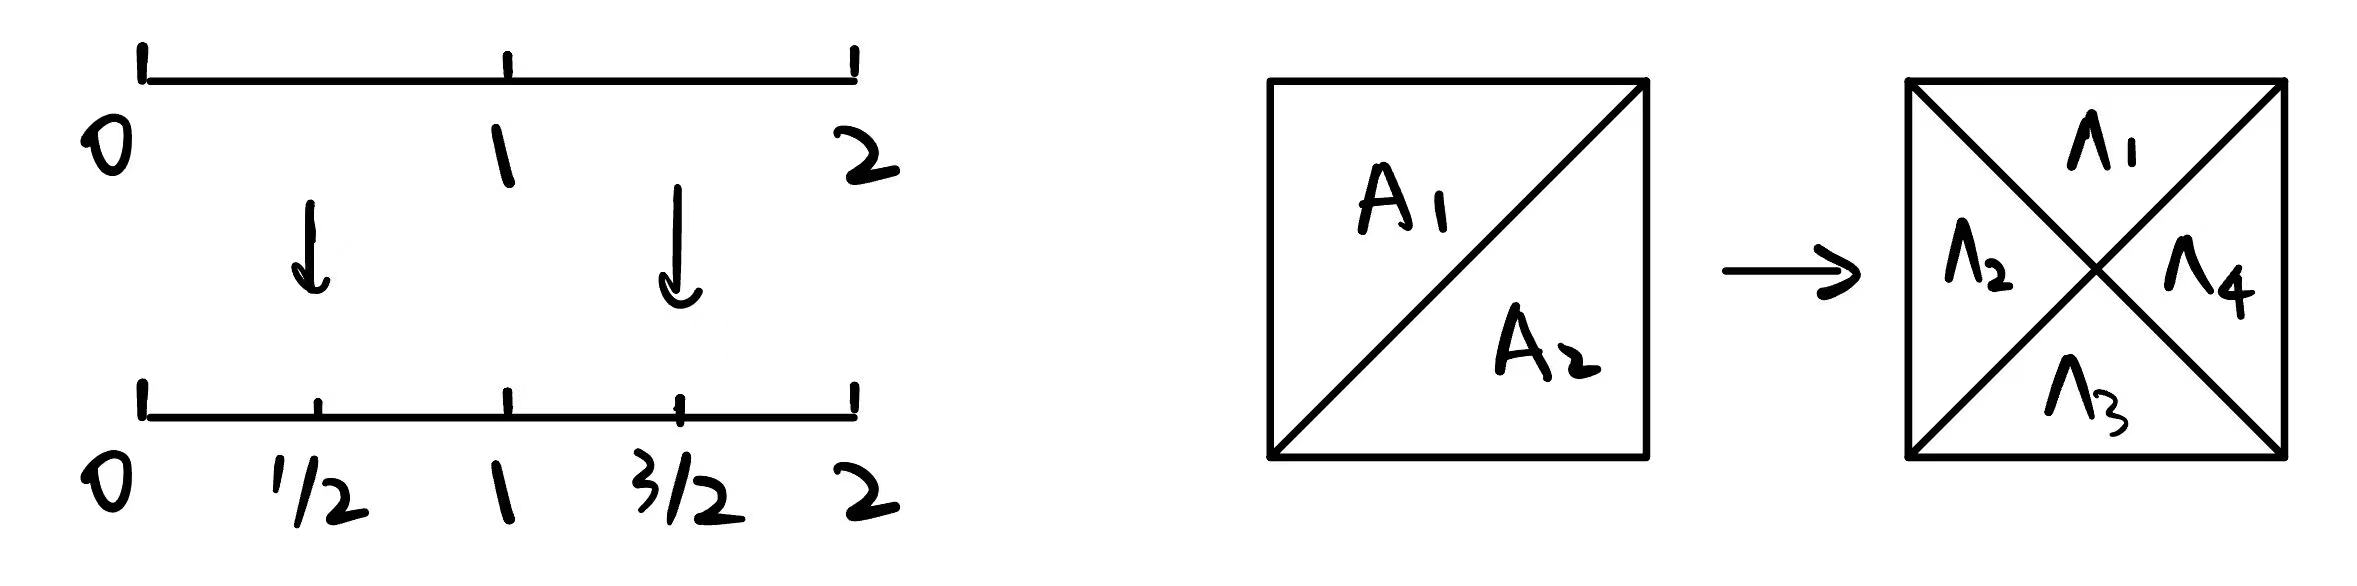
\includegraphics[width=0.8\textwidth]{figures/加细划分.jpg}
    \caption{加细划分}
\end{figure}

(Step 2) 对于 $\omega\in \Lambda_j,\forall j\geq 1$
\[
\begin{aligned}
    \EE(XY|\sigma(\Pi))(\omega) &= \EE(\sum_{k\geq 1}x_k\II_{\Lambda_k}Y|\sigma(\Pi))(\omega)\qquad [X=\sum_{k\geq 1}x_k\II_{\Lambda_k}]\\
    &=\EE(\sum_{k\geq 1}x_k\II_{\Lambda_k}Y|\Lambda_j)\qquad [\sigma(\Pi)\text{定义}]\\
    &=\EE(\sum_{k\geq 1}x_k\II_{\Lambda_k}Y\II_{\Lambda_j})/\PP(\Lambda_j)\qquad [\text{推论\eqref{cor:con_exp_indic}}]\\
    &=\EE(Yx_j\II_{\Lambda_j})/\PP(\Lambda_j)\qquad [\II_{\Lambda_k}\II_{\Lambda_j}\text{当}\Lambda_k\neq\Lambda_j\text{时}=0]\\
    &=x_j\EE(Y\II_{\Lambda_j})/\PP(\Lambda_j)\\
    &=x_j \EE(Y|\II_{\Lambda_j})\\
    &=X(\omega)\EE(Y|\II_{\Lambda_j})
\end{aligned}
\]

\[
\Rightarrow \EE(XY|\sigma(\Pi))=X\sum_{j\geq 1}\II_{\Lambda_j}\EE(Y|\Lambda_j)=X\EE(Y|\sigma(\Pi))
\]

数学上有种现象叫“法国人的伎俩”,即把定理当定义用。严格地讲,这么做有时会出现存在性和唯一性不满足的问题。下面介绍一个常被当做定义用的定理:

\begin{theorem}\label{thm:partition_con_exp}
    $\Pi=\{\Lambda_k,k\geq 1\}$ 为 $\Omega$ 的划分, $\EE|X|<\infty$。记 $Y:=\EE(X|\sigma(\Pi))=\sum_{k\geq 1}\II_{\Lambda_k}\EE(X|\Lambda_k)$,则
    \begin{enumerate}
        \item $Y$ 仍是一个离散随机变量,且 $\EE|Y|\geq \EE|X|<\infty$
        \item $\sigma(Y)\st \sigma(\Pi)$ (记作 $Y\in \sigma(\Pi)$,即 $Y$ 的所有信息都在 $\sigma(\Pi)$ 里)
        \item $\forall A\in \sigma(\Pi)$,有 $\EE(Y\II_A)=\EE(X\II_A)$
    \end{enumerate}
\end{theorem}

证明:(1)$E|X|=\sum_{x\in S_x}|x|\PP(X=x)<\infty$

\[
    \EE|Y|=\sum_{k\geq 1}|\EE(X|\Lambda_k)|\PP(\Lambda_k)\geq \sum_{k\geq 1}\sum_{x\in S}|x|\PP(\{X=x\}\cap \Lambda_k)
\]

逻辑上,现在第一个等号不成立,但之后 $<\infty$ 一写出来,之前的所有等号立刻成立,此处只为书写简便

\[
    \EE|X|=\sum_{x\in S_x}|x|\PP(X=x)=\sum_{x\in S}|x|\sum_{k\geq 1}\PP(\Lambda_k\cap \{X=x\})
\]

我们知道 $\sum_{x\in S}|x|\sum_{k\geq 1}\PP(\Lambda_k\cap \{X=x\})$ 绝对收敛,若求和次序交换后的 $\sum_{k\geq 1}\sum_{x\in S}|x|\PP(\{X=x\}\cap \Lambda_k)$ 也绝对收敛,则 $\EE|Y|<\infty$ 得证。有一个引理可以保证绝对收敛:

\begin{lemma}[\cite{calculus}.P280.推论]\label{lem:abs_convergence}
    从 273-280
\end{lemma}

\begin{corollary}[来自定理\ref{thm:partition_con_exp}(1)]\label{cor:double_exp}
    \begin{enumerate}
        \item (重期望公式)$\EE|\EE(X|\sigma(\Pi))|=\EE|X|, \EE(\EE(X|\sigma(\Pi)))=\EE(X)$
        \item $|\EE(X|\Lambda_k)|\leq \EE(|X|\mid\Lambda_k), |\EE(X|\sigma(\Pi))|\leq \EE(|X|\mid\sigma(\Pi))$
    \end{enumerate}
\end{corollary}

(2) 由定义,$Y=\sum_{k\geq 1}y_k\II_{\Lambda_k}$,其中 $y_k:=\EE(X|\Lambda_k)$

记 $S_Y=\cup_{k\geq 1}\{y_k\}$,注意到,可能 $\exists i\neq j$,但 $y_i=y_j$

故 $J_y=\{k|y_k=y\}(y\in S_Y)$ 中个数可能大于1

\[
Y=\sum_{y\in S_Y}y\II_{\sum_{k\in J_y}\Lambda_k}
\]

\[
\{Y=y\}=\sum_{k\in J_y}\Lambda_k\in \sigma(\Pi)
\]

\[
\sigma(Y)\st \sigma(\Pi)\qed
\]

(3) $\EE(Y\II_A)=\EE(\II_A\EE(X|\sigma(\Pi)))$

\[
\begin{aligned}
    \EE(Y\II_A)&=\EE(\II_A\EE(X|\sigma(\Pi)))\\
    &=\EE(\EE(X\II_A|\sigma(\Pi)))\qquad [A\in \sigma(\Pi), \text{性质\eqref{prt:extract_known}}]\\
    &=\EE(X\II_A)\qquad [\text{重期望-推论\eqref{cor:double_exp}}]
\end{aligned}
\]

\subsubsection*{$3^\circ$关于离散随机变量的条件期望}

\begin{definition}
    概率空间 $(\Omega,\CF,\PP)$,$X,Y$ 为离散随机变量,$\EE|X|<\infty$。定义 $\EE(X|Y)=\EE(X|\sigma(Y))=\EE(X|\sigma(\Pi_Y))$,称为 $X$ 关于 $Y$ 的条件期望
\end{definition}

注:$\omega=\{Y=y\}\in \Pi_Y$ 或 $Y(\omega)=y$,$\EE(X|Y)(\omega)=\EE(X|Y=y)$

\begin{example}
    $\EE(X|\Pi_{\Omega})=\EE(X|\sigma(\Omega))=\EE(X)$
\end{example}

\begin{example}
    $\II_A\ind \II_B\Rightarrow \EE(\II_A|\II_B)=[\text{Exa\eqref{exa:con_exp_indic}}]\EE(\II_A)$
\end{example}

\begin{example}
    $\EE(X|X)=\EE(X|\sigma(X))=X$[\text{Exa \ref{exa:extract_known}}]
\end{example}

\begin{property}
    假设以下期望、条件期望都有意义
    \begin{enumerate}
        \item $\EE(aX+bY|Z)=a\EE(X|Z)+b\EE(Y|Z)$
        \item $X\ind Y\Rightarrow \EE(X|Y)=\EE(X)$
        \item $\sigma(X)\st \sigma(Z)\Rightarrow \EE(XY|Z)=X\EE(Y|Z)$
        \item $\EE(\EE(X|Z))=\EE(X)$
        \item $|\EE(X|Z)|\leq \EE(|X|\mid Z)$
    \end{enumerate}
\end{property}

\subsubsection*{$4^\circ$关于多个离散随机变量的条件期望}

$\EE(Y|X_1,\cdots,X_n)$

\begin{enumerate}
    \item 由 $X_1,\cdots ,X_n$ 生成的 $\sigma$代数 $\sigma(X_1,\cdots,X_n)$
    \item $:=\EE(Y|\sigma(X_1,\cdots ,X_n))$
\end{enumerate}

怎样生成 $\sigma$代数可以包含 $X_1,\cdots,X_n$ 尽可能多的信息?

直觉是 $\bigcup_{k=1}^{\infty}\sigma(X_k)$,然而它不一定是 $\sigma$代数,因为它对可列并不封闭。

每个 \(\sigma(X_k)\) 是一个 \(\sigma\)代数,因此它对可列并封闭。

然而,\(\bigcup_{k=1}^{\infty} \sigma(X_k)\) 只是将每个 \(\sigma(X_k)\) 中的集合简单地并在一起,并没有保证这些集合的可列并仍然在 \(\bigcup_{k=1}^{\infty} \sigma(X_k)\) 中。

例如,假设 \(X_k \in \sigma(X_k)\),那么 \(X_k\) 在 \(\bigcup_{k=1}^{\infty} \sigma(X_k)\) 中,但 \(\bigcup_{k=1}^{\infty} X_k\) 可能不在 \(\bigcup_{k=1}^{\infty} \sigma(X_k)\) 中,因为它可能不属于任何一个单独的 \(\sigma(X_k)\)。问题出在 \(\bigcup_{k=1}^{\infty} \sigma(X_k)\) 缺少 $\{\sigma(X_k)\}_{k\geq 1}$ 交互的部分

怎样把 \(\bigcup_{k=1}^{\infty} \sigma(X_k)\) 变成$\sigma$代数?

\begin{definition}[多个离散随机变量的条件期望]\label{def:multi_rv_con_exp}
    定义由离散随机变量 $X_1,\cdots,X_n$ 生成的 $\sigma$代数
    \[
    \begin{aligned}
        \sigma(X_1,\cdots,X_n)&:=(X_1,\cdots,X_n)^{-1}(2^{S_1}\times \cdots \times 2^{S_n})\\
        &:=\{\underbrace{(X_1,\cdots,X_n)^{-1}(A_1\times\cdots\times A_n)}_{\text{柱集}}|A_1\times\cdots\times A_n\st \underbrace{S_1\times\cdots\times S_n}_{\text{乘积空间}}\}\\
        &=\{\bigcap_{k=1}^{\infty}X_k^{-1}(A_k)|A_k\in 2^{S_k},1\leq k\leq n\}
    \end{aligned}
    \]
\end{definition}

\begin{theorem}\label{thm:discrete_rv_partition}
    令 $x_k=\sum_{i\geq 1}x_{k,i}\II_{\Lambda_{k,i}}, 1\leq k\leq n$,为离散随机变量,对每一个 $k$,$\Pi_k:=\{\Lambda_{k,i}|i\geq 1\}$ 为 $\Omega$ 的划分,定义
    \[
    \Pi_{(X_1,\cdots,X_n)}:=\{\Lambda_{1,i_1}\cap\cdots \cap \Lambda_{n,i_n}|i_k\geq 1,1\leq k\leq n\}
    \]
    则
    \begin{enumerate}
        \item $\Pi_{(X_1,\cdots,X_n)}$ 是 $\Omega$ 的划分,且
        \[
            \sigma(\Pi_{(X_1,cdots,X_n)})=\left \{\sum_{\substack{(i_1,\cdots ,i_n) \\ \in J_1\times \cdots \times J_n}} (\Lambda_{1,i_1}\cap \cdots \cap \Lambda_{1,i_n})|J_k\st \NN,1\leq k\leq n\right \}
        \]
        \item $\sigma(X_1,\cdots,X_n)=\sigma(\Pi_{(X_1,\cdots ,X_n)})$(即定义\ref{def:multi_rv_con_exp}是有意义的,well-defined,make sense,良定义)
    \end{enumerate}
\end{theorem}

\begin{problem}[作业2-2]
    证明定理\ref{thm:discrete_rv_partition}在 $n=2$ 时成立
\end{problem}

\begin{definition}
    $\EE|Z|<\infty$ 定义
    \[
    \EE(Z|X_1,\cdots,X_n)=\EE(Z|\sigma(X_1,\cdots,X_n)):=\EE(Z|\sigma(\Pi_{(X_1,\cdots,X_n)}))
    \]
\end{definition}

\begin{definition}\label{def:multi_rv_indep}
    $(\Omega,\CF,\PP), Y:\Omega\to S_Y, X_1:\Omega\to S_1,X_2:\Omega\to S_2$ 为离散随机变量,称 $Y$ 和 $(X_1,X_2)$ 独立,若 $\sigma(Y)\ind \sigma(X_1,X_2)$. [$\sigma(Y)=Y^{-1}(2^{S_Y}),\sigma(X_1,X_2)=(X_1,X_2)^{-1}(2^{S_1}\times 2^{S_2})$]

    即 $\forall A\st S_Y,B\st 2^{S_1}\times 2^{S_2}, B=B_1\times B_2$,有 
    \[
    \PP(Y\in A,(X_1,X_2)\in B)=\PP(Y\in A)\PP((X_1,X_2)\in B)
    \]
    其中 $\PP((X_1,X_2)\in B)=\PP(X_1\in B_1,X_2\in B_2)$
\end{definition}

\begin{problem}[作业2-3]
    证明:
    \[
    \begin{aligned}
        Y\ind (X_1,X_2)\Leftrightarrow &\forall y\in S_Y,x_1\in S_1,x_2\in S_2\\
        &\text{有}\PP(Y=y,(X_1,X_2)=(x_1,x_2))\\
        &=\PP(Y=y)\PP((X_1,X_2)=(x_1,x_2))
    \end{aligned}
    \]
\end{problem}

有了上述定义,可以推广:

\begin{enumerate}
    \item $(Y_1,\cdots,Y_n)\ind (X_1,\cdots,X_n)$
    \item $Y\ind_A (X_1,\cdots,X_n) (A\in \CF,\PP(A)>0)$
\end{enumerate}

\begin{property}\label{prop:pairwise_indep}
    $Y\ind (X_1,X_2)\Rightarrow Y\ind X_1,Y\ind X_2$
\end{property}

证明:在定义\ref{def:multi_rv_indep}中取$B_2=\Omega$

\[
\begin{aligned}
    \PP(Y\in A,X_1\in B_1)&=\PP(Y\in A,X_1\in B_1,X_2\in S_2)\\
    &=\PP(Y\in A)\PP(X_1\in B_1,X_2\in S_2)\qquad [Y\ind (X_1,X_2)]\\
    &=\PP(Y\in A)\PP(X_1\in B_1)
\end{aligned}
\]

注:看到 $\Rightarrow$ 要自然地问,反过来 $\Leftarrow$ 成立吗?做数学要多问自己一些问题,即便没有答案

\begin{corollary}
    $(Y_1,\cdots,Y_n)\ind (X_1,\cdots,X_n)\Rightarrow Y_k\ind X_j, 1\leq k\leq m,1\leq j\leq n$
\end{corollary}

\subsection{随机过程}

\subsubsection{什么是随机过程}

\begin{definition}[随机过程]
    设 $(\Omega, \CF, \PP)$ 为概率空间,$(S,\CS)$ 为可测空间,$\TT$ 为指标集/参数集,称随机变量族
    \[
    \{X_t: (\Omega,\CF,\PP)\rightarrow (S,\CS)|t\in \TT\}
    \]
    为 (S值) 随机过程 $X$。其中 $(S,\CS)$ 称为 $X$ 的状态空间

    注:\begin{enumerate}
        \item $forall t\in \TT$,$X_t$ 为随机变量
        \item $\TT$ 为时间集,$X_t$ 为过程 $X$ 在时刻 $t$ 的状态
    \end{enumerate}
\end{definition}

\[
\begin{array}{c|cc}
    \TT \backslash S \st \RR & \text{离散 }(e.g.\ \NN) & \text{连续 }(e.g.\ \RR,\RR^+) \\ \hline
    \text{可数集 }(e.g.\ \NN,\ZZ) & \multicolumn{2}{c}{\text{离散时间/参数的随机过程}} \\
    \text{连续统 }(e.g.\ [0,T],\RR^+) & \multicolumn{2}{c}{\text{连续时间/参数的随机过程}}
\end{array}
\]

\subsubsection{随机过程的分布}

\begin{enumerate}
    \item $\forall t\in \TT, X_t:\Omega\rightarrow S$ 为随机变量/可测映射
    \item $X: \TT\times \Omega\rightarrow S$ 二元映射
    \item $X:\Omega\rightarrow S^{\TT}$ 其中 $S^{\TT}=\{f|f:\TT\rightarrow \S\}$,$X:\omega\rightarrow X(\omega)=X(\cdot,\omega)$
\end{enumerate}

分布可用有限维分布族刻画

\begin{definition}
    固定样本点 $\omega$,则 $X_{\cdot}(\omega)$ 为 $\TT\rightarrow S$ 的映射,即 $X_{\cdot}(\omega)\in S^{\TT}$,称 $X_{\cdot}(\omega)$ 是过程 $X$ 的一个实现/样本路径/样本函数
\end{definition}

\begin{definition}
    $\forall n\geq 1, t_1,t_2,\cdots,t_n$ 称 
    \[
    (x_1,x_2,\cdots,x_n)\mapsto F_{t_1,t_2,\cdots,t_n}(x_1,x_2,\cdots,x_n)=\PP(X_{t_1}\leq x_1,\cdots, X_{t_n}\leq x_n)
    \]
    为 $X$ 的 $n$ 维分布
\end{definition}

\begin{definition}[过程的有限维分布族]
    定义
    \[
    \{F_{t_1,t_2,\cdots,t_n}|n\geq 1,t_1,\cdots,t_n\in \TT\}
    \]
\end{definition}

\subsubsection{随机过程的存在性}

\begin{enumerate}
    \item (抽象的) 从概率论/测度论出发去证明随机过程存在性,不写出具体形式,满足随机过程符合给定的有限维分布族即可
    \item (具体的) 构造性证明
\end{enumerate}

\begin{property}
随机过程的有限维分布族具有以下两个性质
\begin{enumerate}
    \item (对称性) 重排,设 $\sigma:\{1,\cdots,n\}\rightarrow \{1,\cdots,n\}$ 为双射,则
    \[
    F_{t_{\sigma(1)}, \cdots,t_{\sigma(n)}}(x_{\sigma(1)},\cdots,x_{\sigma(n)})=F_{t_1,\cdots,t_n}(x_1,\cdots,x_n)
    \]
    \item (相容性) $m\geq n$
    \[
    F_{t_1,\cdots,t_n,t_{n+1},\cdots,t_m}(x_1,\cdots,x_n,+\infty,\cdots,+\infty)=F_{t_1,\cdots,t_n}(x_1,\cdots,x_n)
    \]
    注:相容性类比从高维向低维的投影,$\PP(X\leq +\infty)=F_X(+\infty)=1$
\end{enumerate}
这两个性质是随机过程存在的必要条件
\end{property}

\begin{theorem}[Kolmogorov定理]\label{thm:Kolmogorov}
    设分布函数族
    \[
    \{F_{t_1,\cdots,t_n}|t_1,\cdots,t_n\in \TT,n\geq 1\}
    \]
    满足\uwave{对称性},\uwave{相容性},则必存在一个随机过程 $\{X_t,t\in \TT\}$ 使得上述分布函数族 $F$ 是 $X$ 的有限维分布族
\end{theorem}

\subsubsection{随机过程的基本类型}

\begin{enumerate}
    \item 离散时间马氏链(由条件概率定义)
    \item Poisson 过程
    \item 更新过程
    \item 连续时间马氏链
    \item 离散时间 Martingale (由条件期望定义)
    \item 布朗运动
\end{enumerate}

\begin{definition}
    对连续时间的随机过程 $\{X_t,t\in \TT\}$
    \begin{enumerate}
        \item 若对一切的 $t_0<t_1<\cdots<t_n$ 有 $X_{t_1}-X_{t_0},\cdots,X_{t_n}-X_{t_{n-1}}$ 相互独立,则过程 $X$ 是独立增量过程(e.g. 布朗运动)
        \item 若对每一个 $S\in \TT, X_{t+s}-X_t$ 对一切的 $t$ 都有相同分布,称 $X$ 为平稳增量过程
    \end{enumerate}
\end{definition}